\providecommand{\atlasref}[2]{#2}
\section{Iloczyny, koprodukty i konstrukcje uniwersalne}\label{sec:produkty}

\subsection{Iloczyn}

\begin{definicja}[Iloczyn dwóch obiektów]\label{def:produkt}
Niech $A,B$ będą obiektami kategorii $\mathcal C$. \emph{Iloczynem} $A$ i $B$ nazywamy obiekt $P$ wraz z morfizmami $p_A:P\to A$ i $p_B:P\to B$ o własności: dla każdego obiektu $X$ i każdej pary morfizmów $f:X\to A$, $g:X\to B$ istnieje dokładnie jeden morfizm $\langle f,g\rangle:X\to P$ taki, że $p_A\circ\langle f,g\rangle=f$ i $p_B\circ\langle f,g\rangle=g$.
\end{definicja}

Własność uniwersalną iloczynu przedstawia jeden diagram z dwoma przemiennymi trójkątami; przerywana strzałka $\langle f,g\rangle$ jest jednoznacznie wyznaczona:
\begin{center}
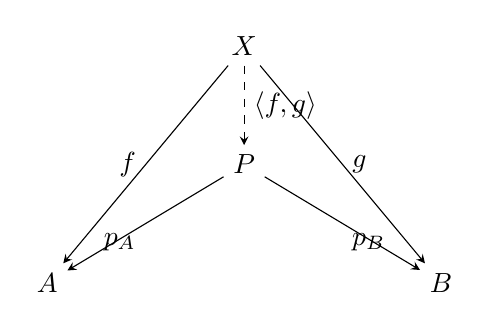
\begin{tikzpicture}[>=stealth]
\node (x) at (0,3) {$X$};
\node (p) at (0,1.5) {$P$};
\node (a) at (-2.5,0) {$A$};
\node (b) at (2.5,0) {$B$};
\draw[->,dashed] (x) -- node[right] {$\langle f,g\rangle$} (p);
\draw[->] (x) -- node[left] {$f$} (a);
\draw[->] (x) -- node[right] {$g$} (b);
\draw[->] (p) -- node[below left] {$p_A$} (a);
\draw[->] (p) -- node[below right] {$p_B$} (b);
\end{tikzpicture}
\end{center}
Przyjmujemy zwykle zapis $P=A\times B$, ale trzeba pamiętać, że chodzi o obiekt z określonymi rzutami, a nie tylko samą klasę izomorfizmu obiektu.

\begin{przyklad}[Zbiory]
W $\Set$ iloczynem jest zbiór par $A\times B$. Unikalna funkcja z definicji ma postać $\langle f,g\rangle(x)=(f(x),g(x))$. W szczególności funkcję do iloczynu można podać, podając osobno obie jej współrzędne.
\end{przyklad}

\begin{przyklad}[Grupy i topologia]
W $\Grp$ iloczynem jest $A\times B$ z mnożeniem $(a,b)(a',b')=(aa',bb')$. W $\Top$ jest nim kartezjański iloczyn wyposażony w topologię produktową. W obu przypadkach uniwersalny morfizm jest odwzorowaniem $h:x\mapsto(f(x),g(x))$. Dla homomorfizmów grup $h(xx')=(f(x)f(x'),g(x)g(x'))=h(x)h(x')$; dla odwzorowań ciągłych przeciwobraz bazowego otwartego prostokąta $U\times V$ wynosi $f^{-1}(U)\cap g^{-1}(V)$, więc jest otwarty. W obu przypadkach rzuty są morfizmami, a ich wartości wyznaczają obie współrzędne $h$, co dowodzi jednoznaczności.
\end{przyklad}

\begin{przyklad}[Iloczyn w przestrzeniach liniowych]
W $\Vect_k$ iloczynem dwóch przestrzeni $V,W$ jest przestrzeń $V\oplus W$ z rzutami na współrzędne. Dla \emph{skończonej} liczby przestrzeni suma prosta i iloczyn prosty są kanonicznie izomorficzne; przy nieskończonej rodzinie należy je rozróżnić.
\end{przyklad}

\begin{przyklad}[Iloczyn w porządku]
W kategorii zbioru częściowo uporządkowanego $P$ iloczyn obiektów $a,b$ istnieje wtedy i tylko wtedy, gdy istnieje ich największe ograniczenie dolne (kres dolny) $a\wedge b$. Rzuty istnieją, bo $a\wedge b\leq a,b$. Każde $x$ spełniające $x\leq a,b$ spełnia $x\leq a\wedge b$. Zatem logiczne \emph{``i''} odpowiada kategorii iloczynu.
\end{przyklad}

\begin{twierdzenie}[Jednoznaczność iloczynu]\label{tw:produkt-unique}
Jeśli $(P,p_A,p_B)$ i $(Q,q_A,q_B)$ są dwoma iloczynami tych samych obiektów $A,B$, to istnieje dokładnie jeden izomorfizm $u:P\to Q$ spełniający $q_A\circ u=p_A$ i $q_B\circ u=p_B$.
\end{twierdzenie}
\begin{proof}
Z własności $Q$ wynika istnienie jedynego $u:P\to Q$ o wymaganych równościach. Z własności $P$ wynika analogicznie istnienie jedynego $v:Q\to P$ zgodnego z rzutami. Teraz $p_A\circ(v\circ u)=q_A\circ u=p_A$ i tak samo dla $p_B$. Ponieważ $\id_P$ również spełnia te dwa równania, jedyność w definicji iloczynu daje $v\circ u=\id_P$. Symetrycznie $u\circ v=\id_Q$.
\end{proof}

\subsection{Koprodukt}

\begin{definicja}[Koprodukt dwóch obiektów]\label{def:koprodukt}
Niech $A,B\in\Ob(\mathcal C)$. \emph{Koprodukt} $A,B$ to obiekt $Q$ z morfizmami $i_A:A\to Q$, $i_B:B\to Q$ taki, że dla każdego $X$ oraz morfizmów $f:A\to X$, $g:B\to X$ istnieje dokładnie jeden $[f,g]:Q\to X$ spełniający $[f,g]\circ i_A=f$ i $[f,g]\circ i_B=g$.
\end{definicja}

Koprodukt jest pojęciem dualnym do iloczynu: definicję otrzymujemy przez odwrócenie wszystkich strzałek, czyli przejście do kategorii przeciwnej. Stosując twierdzenie~\ref{tw:produkt-unique} w $\mathcal C^{\op}$, otrzymujemy jedyny izomorfizm między dwoma koproduktami zgodny z ich morfizmami kanonicznymi.

\begin{przyklad}[Suma rozłączna zbiorów]
W $\Set$ koproduktem jest $A\sqcup B=(A\times\{0\})\cup(B\times\{1\})$, a $i_A(a)=(a,0)$, $i_B(b)=(b,1)$. Dla $f:A\to X$ i $g:B\to X$ jedyna funkcja $[f,g]$ jest określona na obu rozłącznych częściach przez $[f,g](a,0)=f(a)$, $[f,g](b,1)=g(b)$. Nawet gdy $A\cap B\neq\varnothing$, koprodukt zachowuje informacje, z której kopii pochodzi element.
\end{przyklad}

\begin{przyklad}[Koprodukt w grupach]
W $\Grp$ koproduktem jest \emph{iloczyn wolny} $G*H$. Korzystamy z konstrukcji grup wolnych i prezentacji z \atlasref{AA-07::aa:tw:free-exists}{AA-07: istnienie grupy wolnej}. Niech $F$ będzie grupą wolną na rozłącznych kopiach zbiorów $G$ i $H$, a $N$ normalnym domknięciem relacji
\[
[g]_G[g']_G[gg']_G^{-1},\qquad
[h]_H[h']_H[hh']_H^{-1}
\]
dla wszystkich $g,g'\in G$, $h,h'\in H$. Definiujemy $G*H=F/N$. Relacje sprawiają, że odwzorowania $i_G:g\mapsto[g]_GN$ i $i_H:h\mapsto[h]_HN$ zachowują mnożenie, a w szczególności jedynkę (idempotent w grupie jest elementem neutralnym). Dla homomorfizmów $f:G\to K$, $g:H\to K$ własność grupy wolnej daje jedyny homomorfizm $F\to K$ wysyłający oznaczone generatory na ich obrazy przez $f$ i $g$. Każda relacja trafia na jedynkę, więc jądro tego homomorfizmu zawiera $N$ i otrzymujemy homomorfizm $F/N\to K$. Jest jedyny, ponieważ obrazy oznaczonych generatorów generują $F/N$. Wybierając $K=G$, $f=\id_G$ oraz trywialny $g:H\to G$, otrzymujemy lewą odwrotność $i_G$; analogicznie $i_H$ ma lewą odwrotność. Oba morfizmy są więc zanurzeniami grup.

Iloczyn prosty nie realizuje tej własności z kanonicznymi zanurzeniami: weźmy $G=H=\mathbb Z/2\mathbb Z$ i homomorfizmy do grupy permutacji $S_3$, wysyłające generatory odpowiednio na $(12)$ i $(23)$. W $G\times H$ generatory różnych czynników komutują, ale ich zadane obrazy nie komutują. Nie istnieje zatem homomorfizm rozszerzający tę parę.
\end{przyklad}

\begin{przyklad}[Suma prosta przestrzeni]
W $\Vect_k$ koproduktem $V,W$ jest także $V\oplus W$, ale tym razem z zanurzeniami $i_V(v)=(v,0)$, $i_W(w)=(0,w)$. Jedyny morfizm $[f,g]:V\oplus W\to X$ ma wzór $[f,g](v,w)=f(v)+g(w)$. Iloczyn i koprodukt mogą więc mieć ten sam obiekt nośny, lecz są określone przez \emph{inne strzałki i inne własności uniwersalne}.
\end{przyklad}

\begin{przyklad}[Koprodukt w porządku]
Dla kategorii zbioru częściowo uporządkowanego $P$ koprodukt $a,b$ jest ich kresem górnym $a\vee b$, o ile istnieje. Zestawienie przykładów pokazuje dwie kategoryczne wersje słów \emph{``i''} (iloczyn) oraz \emph{``lub''} (koprodukt) w teorii porządku.
\end{przyklad}


\begin{przyklad}[Suma prosta a iloczyn tensorowy]
Niech $V=k^2$ i $W=k^3$. Ich produkt w $\Vect_k$ ma wymiar $2+3=5$; jest nim $V\oplus W$, wyposażony w dwa rzuty. Iloczyn tensorowy $V\otimes_k W$ ma wymiar $2\cdot3=6$, więc nie może być produktem w tej kategorii. Tensor jest opisywany przez \emph{inną} własność uniwersalną: dla każdej przestrzeni $Z$ odwzorowania liniowe $V\otimes_k W\to Z$ są w naturalnej bijekcji z odwzorowaniami dwuliniowymi $V\times W\to Z$. Sama nazwa ``iloczyn'' nie przesądza zatem o konstrukcji kategorialnej.
\end{przyklad}

\begin{przyklad}[Puste produkty i puste koprodukty]
Przyjmując definicję dla rodziny indeksowanej zbiorem (podaną poniżej), iloczyn pustej rodziny obiektów w kategorii $\mathcal C$, jeśli istnieje, to obiekt końcowy: dla każdego $X$ ma istnieć dokładnie jedna strzałka $X\to P$, bo nie ma żadnych rzutów, których zgodność trzeba sprawdzać. Dualnie koprodukt pustej rodziny jest obiektem początkowym. W $\Set$ odpowiadają im odpowiednio singleton i zbiór pusty. To ważny przypadek brzegowy definicji granicy i kogranicy.
\end{przyklad}

\begin{przyklad}[Biprodukt dwóch przestrzeni liniowych]
W $\Vect_k$ dla $V\oplus W$ występują zanurzenia $i_V(v)=(v,0)$, $i_W(w)=(0,w)$ i rzuty $p_V(v,w)=v$, $p_W(v,w)=w$. Spełniają one $p_Vi_V=\id_V$, $p_Wi_W=\id_W$, $p_Vi_W=0$, $p_Wi_V=0$ oraz $i_Vp_V+i_Wp_W=\id_{V\oplus W}$. Ostatnią równość sprawdzamy na $(v,w)$: lewa strona daje $(v,0)+(0,w)=(v,w)$. Te wzory uzasadniają nazwę \emph{biprodukt}: jeden obiekt realizuje jednocześnie produkt i koprodukt, przy ściśle zgodnych zanurzeniach i rzutach.
\end{przyklad}


\subsection{Nie należy mylić istnienia z konstrukcją}

\begin{uwaga}
Nie w każdej kategorii istnieją iloczyny i koprodukty. Dla zbioru częściowo uporządkowanego, w którym dwa elementy nie mają kresu dolnego, odpowiedni iloczyn nie istnieje. Również wtedy, gdy w danej kategorii znamy wygodną konstrukcję na elementach, \emph{własność uniwersalna} jest właściwym narzędziem sprawdzania, czy ta konstrukcja rzeczywiście jest produktem lub koproduktem.
\end{uwaga}

\begin{stwierdzenie}[Zachowanie własności przez izomorfizm]
Jeżeli $(P,p_A,p_B)$ jest iloczynem $A,B$ i $u:Q\to P$ jest izomorfizmem, to $(Q,p_A\circ u,p_B\circ u)$ również jest iloczynem $A,B$. Analogiczne stwierdzenie zachodzi dla koproduktów: jeśli $(P,i_A,i_B)$ jest koproduktem, a $u:P\to Q$ izomorfizmem, to $(Q,u\circ i_A,u\circ i_B)$ jest koproduktem.
\end{stwierdzenie}
\begin{proof}
Dla danych $f:X\to A$, $g:X\to B$ wyznaczmy jedyne $h:X\to P$ zgodne z rzutami. Wtedy $u^{-1}\circ h:X\to Q$ jest zgodny z nowymi rzutami. Jeśli $t:X\to Q$ także jest zgodny, to $u\circ t=h$ na mocy jedyności w $P$, czyli $t=u^{-1}\circ h$. Dla koproduktu, przy danych $f:A\to X$, $g:B\to X$, jedyny morfizm $h:P\to X$ zgodny z $i_A,i_B$ daje morfizm $h\circ u^{-1}:Q\to X$. Każdy inny $t:Q\to X$ zgodny z $u\circ i_A,u\circ i_B$ spełnia $t\circ u=h$, więc $t=h\circ u^{-1}$.
\end{proof}

\subsection{Rodziny dowolnej mocy}

\begin{definicja}[Iloczyn i koprodukt rodziny]\label{cat:def:indexed-products}
Niech $(A_i)_{i\in I}$ będzie rodziną obiektów indeksowaną zbiorem $I$. Iloczyn to obiekt $P$ z rzutami $p_i:P\to A_i$ taki, że każda rodzina $f_i:X\to A_i$ wyznacza jedyny $f:X\to P$ z $p_i\circ f=f_i$ dla wszystkich $i$. Koprodukt to obiekt $Q$ z morfizmami $j_i:A_i\to Q$ taki, że każda rodzina $g_i:A_i\to Y$ wyznacza jedyny $g:Q\to Y$ z $g\circ j_i=g_i$ dla wszystkich $i$. Oznaczamy je odpowiednio przez $\prod_{i\in I}A_i$ i $\coprod_{i\in I}A_i$.
\end{definicja}

W kategorii lokalnie małej własności te odpowiadają bijekcjom
\[
\Hom(X,P)\longrightarrow\prod_{i\in I}\Hom(X,A_i),
\quad f\longmapsto(p_i\circ f)_i,
\]
\[
\Hom(Q,Y)\longrightarrow\prod_{i\in I}\Hom(A_i,Y),
\quad g\longmapsto(g\circ j_i)_i.
\]
Surjektywność jest warunkiem istnienia, a różnowartościowość warunkiem jednoznaczności. Bijekcje są naturalne odpowiednio w $X$ (kontrawariantnie) i $Y$ (kowariantnie): dla $u:X'\to X$ mamy $p_i\circ(f\circ u)=(p_i\circ f)\circ u$, a dla $v:Y\to Y'$ mamy $(v\circ g)\circ j_i=v\circ(g\circ j_i)$. Przy $I=\varnothing$ iloczyn zbiorów morfizmów po prawej stronie jest singletonem, co odzyskuje rozdział~\ref{sec:uniwersalne}.

\begin{przyklad}[Zbiory, grupy i przestrzenie topologiczne]\label{cat:ex:indexed-set-top}
W $\Set$ iloczyn jest zbiorem wszystkich rodzin $(a_i)_{i\in I}$ z $a_i\in A_i$, a koprodukt sumą rozłączną $\{(i,a):i\in I,\ a\in A_i\}$. Dla rodziny funkcji do czynników jedyny morfizm do iloczynu ma wartość $(f_i(x))_i$; do opisu funkcji z koproduktu wystarczy wzór $g(i,a)=g_i(a)$. Dla $I=\varnothing$ są to odpowiednio singleton pustych rodzin i zbiór pusty. Nie zakładamy, że iloczyn niepustych zbiorów jest niepusty bez odpowiedniej postaci aksjomatu wyboru.

W $\Grp$ iloczyn dowolnej rodziny grup ma działanie współrzędne; wzór na morfizm do iloczynu zachowuje mnożenie w każdej współrzędnej.

W $\Top$ na iloczynie zbiorów bierzemy topologię generowaną przez podbazę $p_i^{-1}(U)$, gdzie $U$ jest otwarty w $A_i$ (\atlasref{GT-04::thm:topog-iloczyn-uniwersalnosc}{GT-04: własność uniwersalna iloczynu}). Funkcja $f:X\to\prod_i A_i$ jest ciągła wtedy i tylko wtedy, gdy wszystkie $p_i\circ f$ są ciągłe: w jedną stronę przez składanie, w drugą przez przeciwobrazy podbazy, $f^{-1}(p_i^{-1}(U))=(p_i\circ f)^{-1}(U)$. Na sumie rozłącznej bierzemy topologię, w której $W$ jest otwarty dokładnie wtedy, gdy każde $j_i^{-1}(W)$ jest otwarte. Warunek ten definiuje topologię, gdyż przeciwobrazy zachowują dowolne sumy i skończone przecięcia. Morfizmy $j_i$ są ciągłe, a dla złożonej z $g_i$ funkcji $g$ mamy $j_i^{-1}(g^{-1}(U))=g_i^{-1}(U)$, co dowodzi ciągłości $g$ dokładnie wtedy, gdy wszystkie $g_i$ są ciągłe.
\end{przyklad}

\begin{przyklad}[Iloczyn prosty i suma prosta modułów]\label{cat:ex:module-indexed}
Dla rodziny lewych unitarnych $R$-modułów $(M_i)_{i\in I}$ korzystamy z konstrukcji z \atlasref{AA-16::aa:def:modules-direct-sum}{AA-16: suma prosta i iloczyn prosty modułów}. Iloczyn prosty zawiera wszystkie rodziny elementów, a suma prosta jest podmodułem
\[
\bigoplus_{i\in I}M_i
=\{(m_i)_{i\in I}:\{i:m_i\ne0\}\text{ jest skończony}\}.
\]
Iloczyn prosty jest iloczynem kategorialnym: $x\mapsto(f_i(x))_i$ jest liniowe współrzędnie, a rzuty wymuszają ten wzór. Suma prosta jest koproduktem: dla homomorfizmów $g_i:M_i\to Y$ definiujemy
\[
g((m_i)_i)=\sum_{i\in I}g_i(m_i).
\]
Suma jest skończona, bo $m_i=0$ poza skończonym zbiorem. Addytywność sprawdzamy na skończonej sumie nośników dwóch rodzin, a jednorodność wynika z liniowości wszystkich $g_i$. Ponieważ każdy element sumy prostej jest skończoną sumą elementów z obrazów kanonicznych zanurzeń $j_i$, wzór jest wymuszony warunkami $g\circ j_i=g_i$. Ten sam argument dla grup abelowych wykorzystuje konstrukcję z \atlasref{AA-08::aa:def:abelian-directsum}{AA-08: suma prosta grup abelowych}.

Dla skończonego $I$ oba moduły są równe przy tej realizacji. Dla $I=\mathbb N$ i $M_i=\mathbb Z$ stała rodzina jedynek należy do iloczynu, ale nie do sumy prostej. W szczególności kanoniczna inkluzja sumy prostej w iloczyn nie jest izomorfizmem. Dla $M_i=\mathbb Z/2\mathbb Z$ suma prosta jest przeliczalna (suma zbiorów rodzin o nośniku zawartym w $\{1,\ldots,n\}$), a iloczyn nieprzeliczalny (argument przekątniowy Cantora). W tym przypadku nie istnieje nawet dowolny izomorfizm tych grup.
\end{przyklad}

\subsection{Funktorialność i kanoniczne porównania}

\begin{stwierdzenie}[Iloczyn i koprodukt jako bifunktory]\label{cat:prop:product-functor}
Jeżeli dla każdej pary obiektów kategorii $\mathcal C$ ustalono iloczyn, to przyporządkowanie $(A,B)\mapsto A\times B$ rozszerza się do bifunktora $\mathcal C\times\mathcal C\to\mathcal C$. Analogicznie ustalony koprodukt jest bifunktorem.
\end{stwierdzenie}
\begin{proof}
Dla $f:A\to A'$ i $g:B\to B'$ definiujemy $f\times g$ jako jedyny morfizm $A\times B\to A'\times B'$ z
\[
p_{A'}\circ(f\times g)=f\circ p_A,\qquad
p_{B'}\circ(f\times g)=g\circ p_B.
\]
Rzuty z iloczynu rozróżniają morfizmy do niego. Dla kolejnej pary $f',g'$ złożenie $(f'\times g')\circ(f\times g)$ ma pierwszą współrzędną $f'\circ f\circ p_A$ i drugą $g'\circ g\circ p_B$, tak samo jak $(f'\circ f)\times(g'\circ g)$. Identyczność ma wymagane rzuty, więc $\id_A\times\id_B=\id_{A\times B}$.

Dla koproduktu definiujemy $f\sqcup g$ warunkami $(f\sqcup g)\circ j_A=j_{A'}\circ f$ i $(f\sqcup g)\circ j_B=j_{B'}\circ g$. Po złożeniu kolejnych dwóch takich morfizmów ich ograniczenia wzdłuż $j_A,j_B$ wynoszą $j_{A''}\circ f'\circ f$ i $j_{B''}\circ g'\circ g$. Jednoznaczność dla koproduktu daje zachowanie składania; identyczność spełnia oba warunki dla pary identyczności.
\end{proof}

\begin{stwierdzenie}[Łączność, symetria i jednostka]\label{cat:prop:product-coherence}
W kategorii z ustalonymi iloczynami binarnymi i obiektem końcowym $T$ istnieją kanoniczne izomorfizmy
\[
(A\times B)\times C\cong A\times(B\times C),\quad
A\times B\cong B\times A,\quad A\times T\cong A.
\]
Są naturalne w występujących obiektach. Analogiczne izomorfizmy dla koproduktów otrzymujemy przy obiekcie początkowym.
\end{stwierdzenie}
\begin{proof}
Oba nawiasowania iloczynu trzech obiektów mają trzy rzuty (złożone z odpowiednich rzutów binarnych). Dla dowolnych $f:X\to A$, $g:X\to B$, $h:X\to C$ jedyne morfizmy zgodne z trzema rzutami to odpowiednio $\langle\langle f,g\rangle,h\rangle$ i $\langle f,\langle g,h\rangle\rangle$. Własność iloczynu daje więc w obu kierunkach jedyne porównania zgodne z trzema rzutami. Ich złożenia zachowują wszystkie rzuty, więc są identycznościami. Zamiana kolejności czynników daje porównanie $\langle p_B,p_A\rangle$; zamiana powtórna zachowuje oba rzuty. W przypadku $A\times T$ rzut $p_A$ ma odwrotność $\langle\id_A,!_A\rangle$, gdzie $!_A:A\to T$ jest jedynym morfizmem. Pierwsze złożenie jest identycznością na $A$, a drugie zachowuje rzut na $A$ oraz jedyny morfizm do $T$, więc jest identycznością na $A\times T$.

Dla naturalności każdego porównania składamy obie strony odpowiedniego kwadratu z rzutami na pojedyncze czynniki docelowe. Z definicji morfizmów iloczynowych obie strony dają w każdej współrzędnej ten sam morfizm czynnikowy złożony z odpowiednim rzutem źródłowym. Jednoznaczność iloczynu daje przemienność kwadratu; dla jednostki wystarczy rzut na $A$. W kategorii przeciwnej ten sam argument daje tezy dla koproduktów.
\end{proof}

\begin{stwierdzenie}[Porównanie koproduktu z iloczynem w kategorii z zerami]\label{cat:prop:coprod-product}
Jeżeli $\mathcal C$ ma obiekt zerowy oraz iloczyn $A\times B$ i koprodukt $A\sqcup B$, istnieje kanoniczny morfizm $c:A\sqcup B\to A\times B$ wyznaczony przez
\[
c\circ j_A=\langle\id_A,0_{A,B}\rangle,\qquad
c\circ j_B=\langle0_{B,A},\id_B\rangle.
\]
Nie musi on być izomorfizmem.
\end{stwierdzenie}
\begin{proof}
Oba morfizmy po prawej stronie istnieją przez własność iloczynu i definicję zer z rozdziału~\ref{sec:uniwersalne}. Własność koproduktu daje jedyny $c$. W kategorii modułów dla dwóch czynników jest to identyczność przy realizacji przez pary. W kategorii grup jest to morfizm $G*H\to G\times H$ wysyłający czynniki na odpowiednie podgrupy. Dla $G=H=\mathbb Z/2\mathbb Z$ nie jest iniekcją: komutator generatorów przechodzi na jedynkę, ale sam nie jest jedynką, ponieważ homomorfizm do $S_3$ skonstruowany wcześniej wysyła go na niejednostkowy komutator $(12)(23)(12)^{-1}(23)^{-1}$. Zatem $c$ nie jest izomorfizmem.
\end{proof}

W kategoriach addytywnych wrócimy do warunku, kiedy ten morfizm jest izomorfizmem (biprodukt). Sama obecność obiektu zerowego nie wystarcza.

